\chapter{Clasificación Tradicional}
\label{anexo:clasificacion_tradicional}

\section{Aprendizaje Automático}

El aprendizaje automático, también conocido por su término en inglés
\comillas{\textit{Machine Learning}}, se enmarca dentro del área de la
\acrfull{ia} y estudia cómo las computadoras pueden \comillas{aprender} o
mejorar su rendimiento meramente a partir de datos y sin la intervención de un
ser humano.  La idea detrás de esta disciplina es lograr reconocer patrones
subyacentes en los datos y tomar decisiones basándose en ellos. Por ejemplo, un
problema de aprendizaje automático es el de reconocer dígitos escritos a mano a
partir de un conjunto de ejemplos (ver figura~\ref{fig:reconocimiento_digitos}).
Aquí se tienen un conjunto de imágenes, cada una representando un dígito del 0
al 9, y el objetivo es construir un modelo que sea capaz de detectar de qué
dígito se trata. Otro ejemplo es el de hallar documentos de texto que son
relevantes a una consulta del usuario. En este caso el modelo recibe un conjunto
acotado de términos, los cuales describen una necesidad de información del
usuario, y el modelo debe ser capaz de retornar los documentos que satisfacen la
consulta.

Estos problemas se suelen categorizar en aprendizaje supervisado o no
supervisado, de acuerdo a si se conoce o no de antemano el concepto o etiqueta
que define a los datos. Se desarrollará más sobre este punto en las próximas
secciones. De entre los problemas de aprendizaje supervisado se destaca aquí el
de clasificación, el cual será descrito a continuación.

\begin{figure}
	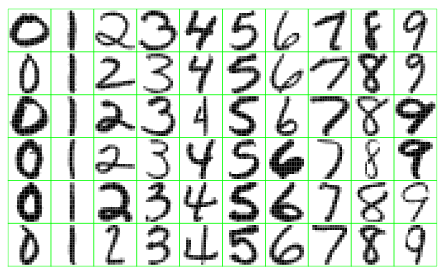
\includegraphics[width=0.66\linewidth]{figures/digits_recognition_v2.png}
	\centering
	\caption[Dígitos escritos a mano.]{Dígitos escritos a mano. Fuente: \citetitle{hastie_elements_2009}
		(\citeyear{hastie_elements_2009}).}
	\label{fig:reconocimiento_digitos}
\end{figure}

\section{Clasificación}

\subsection{Definición}
\label{clasificacion}

La clasificación es una tarea de minería de datos muy popular que consiste en
hallar modelos que describen la o las clases intrínsecas de los datos. La clase
corresponde a un concepto que representa al dato y es una etiqueta categórica,
es decir, un valor discreto de entre un conjunto de valores previamente
conocidos. Estos modelos, también llamados clasificadores, son capaces de
predecir la clase a la que corresponden datos previamente desconocidos. Por
ejemplo, se puede construir un modelo de clasificación para categorizar nuevos
correos electrónicos  de acuerdo a si se trata de correo basura (también
conocido como \comillas{\textit{spam}}) o no. Dicho análisis puede ayudar a
obtener un mayor entendimiento de los datos a alto nivel. Las tareas de
clasificación han sido aplicadas en áreas tales como las de aprendizaje
automático, reconocimiento de patrones o estadística.

En un principio, buena parte de los algoritmos se ejecutaban en memoria, con la
limitación de espacio de almacenamiento que eso conlleva. Investigaciones más
recientes han desarrollado técnicas para escalar los algoritmos de tal manera
que puedan manejar datos de mayor tamaño, alojados en memoria, en disco o
procesados bajo demanda. Las aplicaciones para este tipo de tareas son numerosas
y entre ellas se encuentran las de detectar fraudes o realizar diagnósticos
médicos, entre otras.

La clasificación de datos consta de dos etapas, una de aprendizaje y otra de
clasificación o predicción. Durante la tarea de aprendizaje se construye el
modelo de clasificación  el cual describe un determinado número de clases o
conceptos. También se conoce esta etapa como la de entrenamiento, ya que se
selecciona un subconjunto de los datos, llamado conjunto de entrenamiento, que
consta de instancias o tuplas seleccionadas aleatoriamente y con una o más
etiquetas asociadas. Formalmente, el problema de clasificación puede ser
formulado de la siguiente manera. Se recibe un conjunto etiquetado de
instancias, tupas o ejemplos de la forma $( X, y )$ donde cada tupla es un
vector $X=(x_{1},x_{2},\dots,x_{n})$, siendo cada valor una característica
distintiva, atributo o \textit{feature} de la instancia. El vector $y$ por su
parte toma un valor de entre $n$ clases diferentes.

Este tipo de tareas se engloban dentro del campo de aprendizaje supervisado ya
que para cada instancia la etiqueta es conocida de antemano, y es aprovechada
para guiar o, siguiendo la metáfora, \comillas{supervisar} el aprendizaje del
clasificador. Esta es la diferencia principal contra algoritmos de aprendizaje
no supervisado, en los cuales la etiqueta no es conocida y se deben aplicar
técnicas para salvar esta restricción.

La primera etapa de una clasificación puede ser vista también como el
aprendizaje de una función $y=f(X)$ que pueda predecir la clase $y$ para una
tupla $X$. Por ejemplo, $X$ podría ser un mensaje de correo y la etiqueta $y$ la
decisión de si se trata de un correo basura o no. Desde esta perspectiva
queremos aprender una función que sea capaz de distinguir las clases
subyacentes.  Usualmente, esta asociación es llevada a cabo por algoritmos de
aprendizaje, los cuales internamente usan funciones matemáticas o reglas de
decisión que les permiten procesar los atributos de entrada y generar una salida
acorde. Algunos ejemplos de este tipo de algoritmos son los árboles de decisión,
\textit{naive} bayes, perceptrón, entre otros. Más adelante se retomará sobre
este punto para describir en detalle algunos algoritmos representativos del
campo.

En la segunda etapa el modelo es usado para clasificar y realizar predicciones
sobre datos desconocidos. A este fin, se calcula un valor que refleja la calidad
del clasificador y es denominado \comillas{métrica de evaluación}. Una de ellas
es la exactitud o \textit{accuracy}, pero no es la única.  Durante la etapa de
entrenamiento esta estimación puede ser imprecisa, tomando un valor que tiende a
ser \comillas{optimista} o que da un valor de exactitud mayor al rendimiento
real.  Esto sucede porque el clasificador puede llegar a incorporar anomalías
particulares en el conjunto de datos de entrenamiento, las cuales no tienen que
ver tanto con el dominio de aplicación en el cual se enmarca la tarea, sino más
bien con \comillas{ruido}, datos erróneos o simplemente instancias que no
reflejan correctamente los objetos del mundo real. Este fenómeno es llamado
\comillas{sobreajuste} u \comillas{\textit{overfit}} y se han diseñado técnicas
para reducirlo. Una de ellas consiste en separar de entre los datos de la
colección completa, un subconjunto conocido como \comillas{conjunto de prueba} o
de \textit{testing} que no se usa durante el entrenamiento y a partir del cual
se realizan predicciones y se calculan las métricas de evaluación.

Así pues, la tarea de evaluación es fundamental, ya que es la vía a partir de la
cual se determina qué algoritmos o técnicas son más apropiados que otros para un
problema en particular. Asimismo, provee la información necesaria para corregir
o ajustar los parámetros de los algoritmos y así obtener modelos más robustos.

En definitiva, las etapas de aprendizaje y predicción se aplican
consecutivamente con el objetivo de lograr generar un clasificador capaz de
predecir con éxito las etiquetas de instancias nuevas y a priori desconocidas
por el modelo.

\subsection{Algoritmos}
\label{clasificacion_algoritmos}

Como se mencionó en la sección anterior, una de las etapas de la clasificación
consiste en generar un modelo capaz de clasificar instancias no observadas. En
esta etapa de aprendizaje, se pueden aplicar diversos tipos de algoritmos de
clasificación de acuerdo a la naturaleza de la tarea en particular que se desea
abordar. A continuación, se describen algunos de estos algoritmos en detalle a
fin de ahondar sobre el concepto de clasificación en el aprendizaje automático.
Además, más adelante estos algoritmos serán particularmente relevantes para el
desarrollo del presente trabajo de investigación.

\subsubsection{\textit{Naive} Bayes}

\textit{Naive} Bayes es uno de los algoritmos que pertenecen a la familia de
clasificadores probabilísticos y se destaca por ser computacionalmente simple,
interpretación, y al mismo tiempo brinda un  rendimiento competitivo en
comparación con otros modelos más complejos. Se dice que es un clasificador
estadístico porque se basa en el teorema de Bayes. La idea es computar una
probabilidad para cada una de las clases, basada en los atributos de la
instancia y seleccionar aquella de mayor probabilidad. El término
\comillas{\textit{naive}} es el inglés para el término
\comillas{\textit{ingenuo}} y nace de la presunción que hace el algoritmo de que
los atributos son independientes entre sí, o condicionalmente independientes.
Esta presunción raramente se cumple en los escenarios donde se aplica, pero
contribuye a su simplicidad computacional y a su velocidad durante el
entrenamiento.

Para entender cómo funciona este algoritmo, es bueno abordar primero  el teorema
de Bayes. Formalmente, se define de la siguiente manera:

\begin{equation}
	P(H \mid X) = \frac{P(X \mid H) P(H)}{P(X)}
\end{equation}

En esta ecuación, el vector $X$ es una tupla definida tal como en la sección
anterior y en términos bayesianos representa la \comillas{evidencia}. $P(X)$,
por lo tanto, es la probabilidad de que la tupla contenga los atributos que
efectivamente posee. Por su parte, $H$ es la hipótesis de que la tupla pertenece
a una determinada clase y $P(H)$ su probabilidad. Esta es conocida como
probabilidad \comillas{a priori}. De la misma manera, $P(H|X)$ es la
probabilidad de que la hipótesis $H$ sea cierta bajo la evidencia $X$. A esta se
la llama probabilidad \comillas{a posteriori} con $H$ condicionada por $X$ y es
el valor que se quiere determinar en una tarea de clasificación.  Finalmente,
$P(X|H)$ indica la probabilidad de que la tupla tenga unos atributos
determinados dado que se satisface la hipótesis.

A partir de dicha definición, y de forma similar, se expresa la ecuación de
\textit{Naive} Bayes de la siguiente manera:

\begin{equation}
	P(C_{i} \mid X) = P(X \mid C_{i}) P(C_{i})
\end{equation}

Aquí el término $P(X)$ es descartado porque se asume constante para todas las
clases. La hipótesis $H$ es representada como $C_{i}$ que es un valor de la
tupla $C=(C_{1},C_{2},\dots,C_{q})$, donde $q$ es el número de clases. La
presunción \comillas{ingenua} es aplicada para el cálculo del término $P(X \mid
	C_{i})$ gracias a lo cual se puede definir de la siguiente manera:

\begin{equation}
	P(X \mid C_{i}) = \prod\limits_{k=1}^n{P(x_{k} \mid C_{i})} =
	P(x_{1} \mid C_{i}) \times
	P(x_{2} \mid C_{i}) \times \dots, \times
	P(x_{n} \mid C_{i})
\end{equation}

Finalmente, el modelo seleccionará la clase que maximice el valor de
probabilidad y esa será la salida final del algoritmo.

Como se ha dicho anteriormente, la simplicidad, velocidad computacional y su
competitividad en métricas de exactitud hacen de \textit{Naive} Bayes un
algoritmo destacado en el campo de aprendizaje automático
\cite{wickramasinghe_naive_2020} y ha sido aplicado para problemas diversos,
tales como el de hallar errores en programas de computación
\cite{arar_feature_2017}, predecir enfermedades del corazón
\cite{dulhare_prediction_2018} o detectar ataques en una red de computadoras
\cite{kalutarage_detecting_2015}.


\subsubsection{Árboles de Decisión}

Árboles de decisión es un modelo de clasificación que se destaca por ser de
fácil interpretación e intuitivo para el ser humano. De hecho, se puede generar
una representación gráfica del árbol generado para asistir a la comprensión del
modelo y así entender a más alto nivel cómo se comporta durante una predicción.
En cuanto a su estructura, un árbol de decisión contiene nodos, cada uno
representando un atributo de la colección. Estos nodos se conectan con otros
nodos a partir de enlaces o \comillas{ramas} que representan un valor o un rango
de valores de ese atributo.  Los nodos de menor jerarquía son llamados
\comillas{hojas} y contienen la clase de la predicción, y el nodo de mayor
jerarquía es llamado \comillas{raíz}. Al momento de predecir una instancia
nueva, la clasificación se realiza de la siguiente manera:  se toma la instancia
nueva, la cual no tiene una etiqueta asociada, y los valores de sus atributos
son comparados contra los del árbol, luego se traza un camino desde el nodo raíz
hasta la hoja. Finalmente, la clase que contiene la hoja es seleccionada y será
parte de la predicción resultante.

Los árboles de decisión se generan a partir de un algoritmo de inducción.
Existen varios de estos algoritmos, pero todos son variantes que han sido
diseñadas bajo un mismo principio: construir  el árbol de una manera
\comillas{voraz}\footnote{Se le llama voraz o \textit{greedy} a un algoritmo que
	busca hallar la opción óptima en cada paso y, de esta manera, alcanzar la
	solución general óptima para resolver un problema.  Esto lo diferencia de
	algoritmos como los de \textit{backtracking}, los cuales exploran distintas
	posibilidades y pueden volver al inicio en búsqueda de una mejor solución.},
comenzando desde el nodo raíz (conocido como enfoque \textit{top-down}) y
eligiendo en cada paso el atributo más informativo o que maximice alguna medida
de ganancia de información. Entre estos algoritmos de inducción vale destacar
los siguientes:

\begin{description}

	\item[\acrshort{id3}] Son las siglas de \comillas{\textit{\acrlong{id3}}} y
	      fue desarrollado en 1986 por Ross Quinlan. Consiste en crear un árbol de
	      múltiples vías, buscando para cada nodo el atributo categórico que lance
	      la mayor ganancia de información para las clases categóricas. Los árboles
	      crecen en un tamaño máximo y luego se realiza el paso de poda para mejorar
	      el poder de generalización del modelo sobre datos desconocidos.

	\item[C4.5] Es la evolución del algoritmo \acrshort{id3}. La principal mejora
	      con respecto a su predecesor es que elimina la restricción de que los
	      atributos deban ser categóricos. Esto lo consigue particionando el valor
	      continuo en rangos o en un conjunto de intervalos discretos. A su vez,
	      C4.5 convierte el árbol entrenado en conjuntos de reglas de decisión.

	\item[\acrshort{cart}] Son las siglas de \comillas{\textit{\acrlong{cart}}} y
	      es un algoritmo muy similar al C4.5, pero que soporta clases numéricas, lo
	      cual permite que este algoritmo pueda ser utilizado para resolver
	      problemas de regresión.

\end{description}

Una tarea fundamental en la generación de un árbol es definir un criterio de
división. El objetivo del criterio de división es seleccionar el mejor atributo
en cada paso y existen diversas técnicas para abordar el problema. Una de ellas
es la de \comillas{Ganancia de Información}, usada por el algoritmo
\acrshort{id3}. La técnica de ganancia de información busca seleccionar el
atributo que posee mayor variabilidad o representatividad de los datos y se
sustenta en el cálculo de la entropía o medida de desorden. La idea de fondo es
hallar el atributo que reduzca la entropía esperada. La entropía en el conjunto
de datos $D$ se calcula de la siguiente manera:

\begin{equation}
	Entropia(D) = - \sum_{i=1}^{q} p_{i}\log_{2}(p_{i})
\end{equation}

Nótese que $p_{i}$ corresponde a la probabilidad de que una tupla de $D$
corresponda a la clase $C_{i}$.  A partir de la entropía, se define la ganancia
de información como:

\begin{equation}
	Ganancia(A) = Entropia(D)
	- \sum_{j=1}^{v} \frac{\left\| D_{j} \right\|}{\left\| D \right\|}
	\times Entropia(D_{j})
\end{equation}

Aquí el atributo $A$ divide al conjunto de datos en $v$ particiones, siendo $v$
los valores posibles que toma $A$. $D_{j}$ es el subconjunto de los datos cuyas
tuplas poseen el valor $v$ del atributo $A$, siendo $\left\|D_{j}\right\|$ su
cardinalidad o número de instancias del subconjunto. Al dividir este término por
la cardinalidad del conjunto de datos, se obtiene un valor que representa el
peso de la partición y que es aplicado sobre la entropía esperada. Este proceso
se repite para todos los atributos y, una vez obtenidos los valores de ganancia
para cada uno de ellos, se elige aquel que maximiza la ganancia y finalmente el
atributo seleccionado será el criterio de separación en el nodo.

El algoritmo C4.5 introdujo una mejora en esta técnica llamada \comillas{Razón
	de Ganancia}. La misma busca disminuir uno de los efectos adversos que provoca
la técnica de ganancia de información, esta es, que tiende a favorecer a
atributos con un mayor número de valores posibles. La razón de ganancia, en
primer lugar, reemplaza la fórmula $Entropia(D)$ por la siguiente expresión:

\begin{equation}
	EntropiaRG_{A}(D) = - \sum_{j=1}^{v} \frac{\left\| D_{j} \right\|}{\left\| D \right\|}
	\times \log_{2}(\frac{\left\| D_{j} \right\|}{\left\| D \right\|})
\end{equation}

A partir de allí, el cálculo de la razón de ganancia hace uso de la ganancia y
de la entropía y se formula como:

\begin{equation} \label{eq:gan_c45}
	RazonGanancia(A) = \frac{Ganancia(A)}{EntropiaRG_{A}(D)}
\end{equation}

Finalmente, el atributo de mayor razón de ganancia es seleccionado como criterio
de corte y se continúa el cálculo con los siguientes subnodos.

\subsubsection{Ensambles}
\label{ensambles_intro}

Los ensambles son un conjunto de clasificadores cuyas salidas son combinadas
entre sí con el objetivo de realizar mejores predicciones que cualquiera de
ellos individualmente. En pocas palabras, el enfoque de ensambles consiste en
generar $k$ clasificadores llamados \comillas{clasificadores base}, desde un
mismo algoritmo o no, y entrenarlos con distintos subconjuntos de la colección
de entrenamiento original. Dada una tupla nueva, cada clasificador devuelve su
propia predicción, llamada \comillas{voto}, y luego el ensamble combina cada uno
de estos votos siguiendo algún método de combinación elegido, de forma tal de
producir una predicción final óptima.

La aplicación de ensambles en problemas de clasificación nace de la
imposibilidad de generar un único modelo capaz de generalizar lo suficiente como
para lograr un rendimiento perfecto. Ante la presencia de datos ruidosos,
atípicos o erróneos los clasificadores pueden tender a clasificar mejor para un
subconjunto de datos y no tan bien para otros. Este escenario es aprovechado por
el enfoque de ensambles, ya que su éxito tiene correlación directa con la
existencia de \comillas{diversidad} en la clasificación, distinguiendo el
concepto de diversidad como la existencia de variabilidad entre los modelos,
entre hiperparámetros o entre particiones del conjunto de datos. En definitiva
se entiende que, cuanto mayor es esta diversidad, mayor es la probabilidad de
aislar los posibles errores particulares de un modelo, y al suceder esto, el
error terminará siendo filtrado por el ensamble en la clasificación final. En
consecuencia, se espera lograr una disminución del error total de la
clasificación así como también una mayor exactitud en la predicción, comparando
contra la salida individual de cada clasificador base. Sumado a esto, un
enfoque de ensambles abre la posibilidad de distribuir y/o paralelizar el
cómputo de la predicción, pudiendo así mejorar los tiempos de ejecución durante
el entrenamiento.

En suma, existen distintos tipos de ensamble de acuerdo a su construcción y
arquitectura. A continuación se describen tres de ellos: los ensambles de tipo
\comillas{\textit{bagging}}, los de tipo \comillas{\textit{boosting}} y los de
tipo \comillas{\textit{stacked}}.

\begin{description}

	\item[Bagging] Esta es una de las primeras técnicas de ensambles conocidas y
	      fue introducida por
	      \citeauthor{breiman_bagging_1996}\cite{breiman_bagging_1996}. La misma se
	      desarrolla de la siguiente manera: dado un conjunto de entrenamiento $D$
	      con $n$  tuplas, \textit{bagging} genera un número $m$ de nuevos conjuntos
	      de datos de entrenamiento, cada uno con $n$ tuplas. Para esto se toman
	      tuplas del conjunto original de manera aleatoria y con reemplazo, es decir
	      que puede haber tuplas repetidas y otras que no están incluidas en el
	      nuevo conjunto.  Luego a partir de cada conjunto nuevo, se entrena un
	      clasificador $M_{i}$. Cada clasificador puede ser del mismo tipo porque la
	      diversidad está dada por los datos. En la etapa de clasificación, cada
	      modelo $M_{i}$ genera una predicción que cuenta como un voto. El ensamble
	      cuenta los votos y elige la clase con mayor cantidad de votos, siendo esta
	      la decisión final del ensamble.


	\item[Boosting] En la técnica de \textit{boosting} se asigna un peso a cada
	      tupla de entrenamiento y se generan un conjunto de clasificadores, cada
	      uno a partir del anterior. A diferencia del método de \textit{bagging},
	      \textit{boosting} trabaja siempre sobre el mismo conjunto de datos y la
	      variabilidad está dada por los pesos que son asignados. El proceso es el
	      siguiente: para el primer modelo de clasificación, $M_{i}$, los pesos son
	      inicializados en un mismo valor para todas las tuplas. Una vez que se
	      entrena este modelo, los pesos son actualizados de tal manera que el
	      siguiente clasificador $M_{i} + 1$ trate de manera particular a las tuplas
	      mal clasificadas por $M_{i}$. De ese modo se busca llegar a una
	      clasificación correcta en las sucesivas iteraciones.  Finalmente, el
	      modelo de ensamble combina los votos de cada clasificador individual. Cabe
	      notar que el peso de cada voto también es ponderado de acuerdo al
	      rendimiento del clasificador base.


	\item[Stacking] La técnica de \textit{stacking} fue desarrollada por
	      \citeauthor{wolpert_stacked_1992}\cite{wolpert_stacked_1992} y consiste en
	      entrenar un nuevo clasificador de acuerdo a las predicciones realizadas
	      por otros modelos, tomando la salida de estos modelos como entrada, de tal
	      manera de lograr hallar una combinación que produzca una mejor predicción.
	      Este tipo de ensambles puede ser visto como un conjunto de capas. La
	      primera capa consta de un ensamble de clasificadores que aprenden a partir
	      de los datos de entrenamiento. Esta capa no necesariamente usa
	      clasificadores del mismo tipo, mismos hiperparámetros o particiones de la
	      colección iguales, quedando estos detalles a cargo de quien diseña esta
	      capa. La siguiente capa es el clasificador individual, o
	      meta-clasificador, que se alimenta de las salidas de los clasificadores de
	      la capa inferior y realiza el aprendizaje a partir de las clases
	      producidas por estas salidas y las clases reales.

\end{description}

Una de las tareas a tener en cuenta durante el entrenamiento de un ensamble es
la de combinar las salidas de cada modelo en una salida final. La estrategia más
común y simple es la de votación por mayoría, la cual normalmente es aplicada
por los métodos de \textit{bagging}. No obstante, existen múltiples métodos de
combinar los votos, e incluso no siempre un ensamble de tipo \textit{bagging}
debe aplicar esta estrategia. Por ejemplo, algunos clasificadores pueden decidir
producir una salida solo en el caso de que más de la mitad de ellos coincidan, o
incluso ser más restrictivos y obligar a que la coincidencia sea total. El
enfoque de \textit{boosting} por su parte, pondera al voto de acuerdo a los
pesos que calcula, dando predominio a determinadas instancias.  También se suele
dar un mayor peso a determinados clasificadores por sobre otros. Este tipo de
métodos se los denomina \comillas{votación por mayoría ponderada} y pueden
llevar a un rendimiento superior si es aplicada en el escenario adecuado.

\subsection{Evaluación}
\label{evaluacion_intro}

Llevar a cabo evaluaciones de rendimiento sobre los modelos es un aspecto
importante del aprendizaje automático, ya que nos permite conocer en qué medida
un algoritmo es superior a otro para resolver una tarea. Particularmente, la
tarea de clasificación es un desafío que se presenta en un contexto cambiante y
evolutivo, donde nuevas herramientas surgen y se actualizan constantemente.
Incluso la composición y estructura de los modelos de clasificación varía según
la familia de algoritmos aplicados, y es esperable que los conceptos extraídos
de un modelo de tipo árbol tengan particularidades que lo diferencien de modelos
de redes neuronales o modelos probabilísticos. Y del mismo modo, es esperable
que alguno de estos modelos tenga un mejor rendimiento que otro en un
determinado escenario, o incluso que sea mejor que un modelo generado por el
mismo algoritmo pero con distintos hiperparámetros. La tarea de evaluación es
la que permite detectar estas particularidades y sacar provecho de los
algoritmos para obtener aún mejores modelos.

A su vez, es importante estudiar las métricas de evaluación existentes y llevar
adelante estrategias que nos permitan obtener medidas de evaluación confiables y
que no hayan sido sesgadas por los datos que se usaron durante el entrenamiento.
Y del mismo modo, entender los factores que provocaron un valor de métrica puede
ser el paso inicial para hallar mejoras al modelo que optimizan su capacidad de
predicción en el futuro.

Por consiguiente, a continuación se estudian algunas de las estrategias llevadas
a cabo durante la evaluación para evitar sesgos, así como también las métricas
que se calculan durante este proceso.

\subsubsection{Métricas}
\label{evaluacion_metricas}

Las métricas de evaluación se usan para conocer la habilidad predictiva de un
modelo de clasificación. Se van a describir aquí las métricas más conocidas del
campo y que proveen, a su vez, un primer vistazo de lo que serán las métricas
usadas para evaluar algoritmos para datos multi-etiquetados en las futuras
secciones del escrito.

Antes de comenzar es importante aclarar algunos términos que serán usados para
definir las métricas. Se entiende como \comillas{ejemplos positivos} a aquellas
instancias cuya etiqueta pertenece a la clase de interés en el problema de
estudio y \comillas{ejemplos negativos} como aquellas que no pertenecen a dicha
clase. Al mismo tiempo, se derivan cuatro conceptos que estarán presentes en las
fórmulas para calcular las métricas, los cuales son:

\begin{description}

	\item[\acrfull{vp}] Son los ejemplos positivos que fueron correctamente
	      clasificados como positivos.

	\item[\acrfull{vn}] Son los ejemplos negativos que fueron correctamente
	      clasificados como negativos.

	\item[\acrfull{fp}] Son los ejemplos negativos que fueron incorrectamente
	      clasificados como positivos.

	\item[\acrfull{fn}] Son los ejemplos positivos que fueron incorrectamente
	      clasificados como negativos.

\end{description}

Una vez obtenidos estos conceptos se pueden calcular una serie de métricas a
partir de ellos. Estas métricas son:

\paragraph{Exactitud}
\label{evaluacion_metricas_exactitud}

La exactitud o \textit{accuracy} es la proporción de ejemplos correctamente
clasificados sobre el número total de instancias y a mayor el valor de exactitud
mejor es el rendimiento del clasificador. Se define  como:

\begin{equation}
	exactitud = \frac{\acrshort{vp} + \acrshort{vn}}{\acrshort{vp} +
		\acrshort{vn} + \acrshort{fp} + \acrshort{fn}}
\end{equation}

\paragraph{Tasa de Error}

A la inversa de la exactitud, la tasa de error es la proporción de ejemplos
incorrectamente clasificados sobre el número total de instancias y a menor el
valor de la tasa de error mejor es el rendimiento del clasificador. Se define
como:

\begin{equation}
	tasaError = \frac{\acrshort{fp} + \acrshort{fn}}{\acrshort{vp} +
		\acrshort{vn} + \acrshort{fp} + \acrshort{fn}}
\end{equation}

\paragraph{Precisión}

La precisión es la proporción de ejemplos que fueron clasificados como positivos
y que efectivamente lo son. Mayor es el valor de precisión mejor es el
rendimiento del clasificador. Se dice que es una medida de exactitud y se define
como:

\begin{equation}
	precision = \frac{\acrshort{vp}}{\acrshort{vp} + \acrshort{fp}}
\end{equation}

\paragraph{Exhaustividad}

La exhaustividad o \textit{recall} es la proporción de ejemplos positivos que
fueron clasificados como positivos. Mayor es el valor de exhaustividad mejor es
el rendimiento del clasificador. Se dice que es una medida de completitud y se
define como:

\begin{equation}
	exhaustividad = \frac{\acrshort{vp}}{\acrshort{vp} + \acrshort{fn}}
\end{equation}

\paragraph{Medida-F1}

La medida-F1 o \textit{f1-score} es una medida que integra las métricas de
precisión y exhaustividad tomando la media harmónica entre ambas. Mayor el valor
de esta medida, mejor es el rendimiento del clasificador. Se define como:

\begin{equation}
	medidaF1 = \frac{2 \times precision \times exhaustividad}
	{precision + exhaustividad}
\end{equation}

Por otro lado, existen métricas para evaluar la eficiencia del clasificador en
términos de velocidad y consumo de memoria. Estas métricas cobran especial
importancia en ambientes de flujos continuos de datos, donde el volumen de datos
es grande, la velocidad en la que arriban es alta y los recursos escasean. A
continuación se añade una breve descripción de ambas.

\paragraph{Velocidad}

La velocidad se refiere al costo computacional de generar el modelo y realizar
predicciones, en general se deja fuera del cálculo los tiempos invertidos en
cargar la colección en memoria, realizar tareas de normalización y
preprocesamiento sobre los datos y otras etapas de la clasificación. A menor el
tiempo de ejecución, mejor es el rendimiento del algoritmo.

\paragraph{Consumo de Memoria}

El consumo de memoria es un indicador de los requerimientos de memoria
aproximados para almacenar el modelo, así como también un indicador de resguardo
para estimar el posible consumo de memoria durante la ejecución y asegurarse que
el algoritmo se mantiene en actividad. A menor el consumo de memoria, mayor es
la eficiencia del modelo.

\subsubsection{Estrategias}
\label{evaluacion_estrategias}

Una vez que se define la métrica o el conjunto de métricas apropiadas para
medir el rendimiento de los clasificadores, el siguiente desafío es seguir un
procedimiento de pruebas capaz de lograr resultados de evaluación que puedan ser
generalizables a conjunto de datos aún no observados. Las técnicas de
\comillas{\textit{Holdout}} y \comillas{Validación Cruzada} son dos de las
técnicas más populares para evaluar la habilidad predictiva de los
clasificadores y se describen a continuación.


\paragraph{\textit{Holdout}}

En este método un conjunto de instancias es separado de la colección y se
reserva para evaluar el rendimiento del clasificador.  Este subconjunto es
distinto del conjunto de datos de entrenamiento usado para generar el modelo y
es llamado \comillas{conjunto de pruebas o \textit{testing}}. Una vez entrenado,
el clasificador recibe las instancias del conjunto de pruebas, pero sin incluir
las etiquetas. La salida del clasificador son las etiquetas de cada instancia.
Finalmente, las etiquetas producidas durante la predicción y las etiquetas
reales de cada instancia se combinan y se calculan las métricas de evaluación.
Esta técnica se basa en la idea de que, separando los datos que se usan durante
el entrenamiento de aquellos usados durante la predicción, se logra una
independencia en los datos que derivará en un mayor grado de generalización en
el modelo.

Por contrapartida, el enfoque de \textit{Holdout} tiene la limitación de que
para lograr generalizar requiere de un número de instancias
considerable~\cite{bifet_machine_2018}. Esta idea proviene del hecho de que muy
pocos datos en el conjunto de entrenamiento puede derivar en predicciones
pobres, pero, por el contrario, muy pocos datos en el conjunto de pruebas
tampoco es recomendable, ya que podría resultar en medidas de rendimiento poco
fiables. A esto se suma una de las dificultades más comunes en el área de
aprendizaje automático: la falta de disponibilidad de colecciones grandes de
datos del mundo real.

Por estas razones, ha tomado peso el uso de técnicas de muestreos de datos para
reutilizar instancias de entrenamiento y de prueba. Una de ellas es la de
validación cruzada.

\paragraph{Validación Cruzada de K iteraciones}

La técnica de validación cruzada, más conocida por el inglés \textit{k-fold
	cross-validation}, consiste en particionar el conjunto de datos en $k$
subconjuntos de manera aleatoria y en la forma $\{d_{1}, d_{2},  \dots, d_{k}
	\}$, siendo cada uno de los subconjuntos mutuamente excluyentes entre sí y de
igual o similar tamaño. El proceso itera sobre cada uno de los subconjuntos para
generar $k$ modelos. En la primera iteración $i$, se separa el subconjunto
$d_{i}$ y se entrena el modelo con los restantes subconjuntos para luego medir
el rendimiento con él. En la segunda iteración, se repite este procedimiento
pero usando como pruebas al subconjunto $d_{i+1}$, y así en cada iteración. Así
pues, cada subconjunto es usado una vez para probar el modelo. Finalmente, se
toman los $k$ modelos generados y se promedian las métricas.

De esta técnica derivan otras similares como \comillas{\textit{leave-one-out}}
en donde cada subconjunto es conformado por $n-1$ instancias, siendo $n$ el
tamaño de la colección, dejando un elemento fuera del subconjunto y que será
usado para validar el modelo. El proceso se repite $n$ veces y se combinan los
modelos tal como en el método de validación cruzada.

Otra técnica similar es la de \comillas{Validación Cruzada Estratificada}, la
cual consiste en generar subconjuntos de entrenamiento y pruebas que respeten la
representación de clases existentes en la colección inicial. Por ejemplo, si una
de las clases del problema aparece en el $25\%$ de las instancias, este método
asegura que al generar las particiones esa clase continuará siendo representada
por el $25\%$ de las tuplas. Esta técnica puede ser útil para problemas donde
existe una diversidad que es necesario reflejar en las particiones para obtener
medidas precisas.

En general, los investigadores recomiendan usar validación cruzada con $k=10$ ya
que se suelen conseguir estimaciones menos sesgadas sin incurrir en costos
computacionales demasiado altos.

